\documentclass{beamer}
%\usepackage[ngerman]{babel}
%\usetheme[background=dark]{m}                     % Use metropolis theme
%\usetheme{theme/beamerthemem}                     % Use metropolis theme
\usetheme{metropolis}                     % Use metropolis theme
\usepackage{multimedia}


\title{The Future of Mobility}
\date{\today}
\author{Some Guy, Some Other Guy}
\institute{FHNW Brugg-Windisch}


\begin{document}
    \maketitle

    % ------------------------------------------------------------------------ %
    \section{Video: Volkswagen Urban Mobility 2030}
    % ------------------------------------------------------------------------ %

    \begin{frame}{Volkswagen Urban Mobility 2030: Video}
        %\movie[externalviewer]{}{volkswagen.mp4}
        \begin{center}
            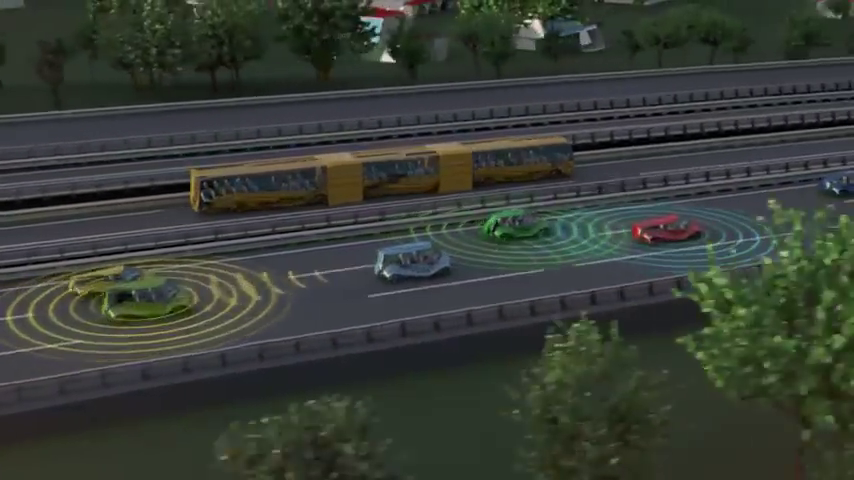
\includegraphics[width=0.8\textwidth]{vw.png}
        \end{center}
    \end{frame}

    \newcounter{enumTemp}

    \begin{frame}{Volkswagen Urban Mobility 2030: Answers}
        \begin{enumerate}[<+-|alert@+>]
            \item
                What is a key issue we are facing when it comes to urban mobility in the near future?
            \item[]
                Limited space, more people, more traffic, people should still be mobile
            \item
                Why does mom leave later?
            \item[]
                The TripManager is networked and acquired the information from the internet.
            \item
                How does the car get current traffic information?
            \item[]
                By car-to-car and car-to-infrastructure communication.
            \item
                How is stop-and-go traffic avoided?
            \item[]
                By keeping optimal gaps between cars.
            \setcounter{enumTemp}{\theenumi}
        \end{enumerate}
    \end{frame}

    \begin{frame}{Volkswagen Urban Mobility 2030: Answers}
        \begin{enumerate}[<+-|alert@+>]
            \setcounter{enumi}{\theenumTemp}
            \item
                How are accidents avoided?
            \item[]
                Every car uses sensors to detect its surroundings, shares that information with other cars and reacts autonomously.
            \item
                How are available parkings spaces optimally utilized?
            \item[]
                Cars have a cooperative parking mode.
            \item
                What is a micro city?
            \item[]
                A node where various modes of transportation come together and various service offerings are in a single place.
            \item
                How is traffic optimized during road works?
            \item[]
                Narrowed lanes.
        \end{enumerate}
    \end{frame}

    % ------------------------------------------------------------------------ %
    \section{Discussion 1}
    % ------------------------------------------------------------------------ %

    \begin{frame}{Discussion 1}
        In groups of 3-5 people discuss the following questions:

        %\begin{itemize}[<+-|alert@+>]
        \begin{itemize}
            \item
                What are advantages/disadvantages of car sharing?
            %\begin{itemize}[<+-|alert@+>]
            %    \item[]
            %    Advantages: always the most suitable car, cars are better utilized, potential for earning money, you pay what you use
            %    \item[]
            %    Disadvantages: availability is not guaranteed, other people might not take good care of your car
            %\end{itemize}
            \item
                Do you think the vision presented in the video is feasible? And if so, how soon?
            \item
                Do you see any downsides to a future as depicted in the video?
        \end{itemize}
    \end{frame}

    % ------------------------------------------------------------------------ %
    \section{Gapped Reading}
    % ------------------------------------------------------------------------ %

    \begin{frame}{The Ethics of Saving Lives: Solutions for Gaps}

        \begin{enumerate}[<+-|alert@+>]
            \item
                cars
            \item
                reflexes
            \item
                deaths
            \item
                right
            \item
                passengers
            \item
                follow
            \item
                security
            \item
                error
        \end{enumerate}
    \end{frame}

    \begin{frame}{The Ethics of Saving Lives: Understanding the Article}
        \begin{itemize}[<+-|alert@+>]
            \item
                An autonomous car always makes the right choice.
            \item[]
                false
            \item
                It is important to think about security and privacy.
            \item[]
                true
            \item
                Autonomous cars can reduce the number of accidents and fatalities.
            \item[]
                true
            \item
                Cars are slower than people at making decisions.
            \item[]
                true
        \end{itemize}
    \end{frame}

    \begin{frame}{The Ethics of Saving Lives: Understanding the Article}
        \begin{itemize}[<+-|alert@+>]
            \item
                What are some flaws of human drivers?
            \item[]
                Can be tired, drunk, emotionally unstable, distracted, ...
            \item
                Why might your car decide to kill you?
            \item[]
                In cases of moral dilemmas, attempting to minimize casualties, encountering a no-win scenarios.
            \item
                Which segment of the population could benefit most from automated cars?
            \item[]
                Disabled and elderly people.
        \end{itemize}
    \end{frame}

    % ------------------------------------------------------------------------ %
    \section{Final Discussion}
    % ------------------------------------------------------------------------ %

    \begin{frame}{Final Discussion}
        \begin{itemize}
            \item
                What is your opinion on the future of mobility?
            \item
                How do you think algorithms for self-driving cars should be regulated, if at all?
            \item
                Do you think people should have a right to drive manually, or should all driving be automated at some point?
            \item
                What do you think will happen outside of the cities, especially in rural areas?
            \item
                Would you like to own a self-driving car?
        \end{itemize}
    \end{frame}

    % ------------------------------------------------------------------------ %
    \section{The End}
    % ------------------------------------------------------------------------ %

\end{document}
